\documentclass[12pt]{article}
\usepackage{times}
\usepackage[backend=biber, isbn=false, doi=false, annotation]{biblatex-chicago}
\bibliography{sources}
\usepackage{amsmath}
\usepackage[margin=1in]{geometry}
\usepackage{
  fancyhdr,
  setspace,
  titlesec,
  graphicx
}
\graphicspath{ {./images/} }
\setstretch{1.5}

\begin{document}

\vspace*{1in} % add star so that vspace is not deleted at beginning of page
\begin{center}
\large{
  \textbf{Development of Quadcopter for Autonomous Navigation and Exploratory Design of Solid State LiDAR}
}
\end{center}

\vspace{1in}

\begin{center}
Simon J. Jones \\
Daniel Willey, PhD \\
Janyl Jumadinova, PhD
\end{center}

\vspace{1in}

\begin{center}
Fall 2023
\end{center}

\vspace{1in}

\begin{center}
\textit{Department of Physics} \\
\textit{Department of Computer and Information Science} \\
\textit{Allegheny College, Meadville, PA 16335}
\end{center}

\newpage

\begin{center}\small{\textbf{ABSTRACT}}\end{center}
\noindent
Here I propose a two-sided project involving the development of a quadcopter capable of autonomous navigation and the exploratory prototype design of a solid state Light Detection and Ranging (LiDAR) system. Many autonomous systems rely on ranging sensors to determine the relative position of obstacles while navigating. LiDAR has numerous applications in robotics, autonomous navigation, and surveying. LiDAR sensor data can be used alone or in tandem with camera data to perform spatial mapping of a robot's environment. \autocite{raj2020} Research in the past decade has made the field of Deep Reinforcement Learning (DRL) infamous for its reduced need for sample data. \autocite{zhu2021} DRL has shown strong potential, especially for autonomous navigation. \autocite{hodge2021} We plan to train a quadcopter for autonomous navigation using a DRL algorithm. The quadcopter will be equipped with a sequence of Time-of-Flight (ToF) sensors as a LiDAR system. Because LiDAR systems are increasingly becoming solid-state, meaning they omit the use of mechanical processes to scan their surroundings,\autocite{li2022} we will also be exploring the novel design of a solid-state LiDAR component for beam deflection by using a nematic Liquid Crystal (LC). We will measure our success by the effectiveness of the quadcopter to navigate through increasingly restricted environments and how large of an angle the LiDAR system can deflect a light source. Additionally, we will compare our results to similar work done in the literature to evaluate our approach to training the quadcopter as well as our implementation of the LiDAR component.

\subsection*{INTRODUCTION \& BACKGROUND}

Robotic navigation is the ability of an autonomous system to determine a course of action to avoid colliding with an obstacle.
Navigation is necessary for a robot to interact with a real world scenario and to realize technologies such as fully autonomous vehicles.
Modern robotics use either ranging sensors (acoustic or optical) or camera information to interpret the relative position of obstacles; however, interpreting reliable and fast 3D spatial data via a camera, called optical flow, requires extensive training and large amounts of data.
Although recent work has enabled a racing quadcopter to outperform professional pilots, boasting a speed of $22\frac{\text{m}}{\text{s}}$ using only an optical flow model, training a model from ranging sensor data is much simpler compared to that of system using a camera for image-based ranging, which is important when considering the feasibility of this project. \autocite{song2023}
Ranging sensors can supply scalar interpretations of the distance between the sensor and the obstacle.
Supplying an array of spatial measurements in the form of a tensor can be used to train a machine learning model capable of avoiding collisions while navigating a robot.
In the past decade, Deep Reinforcement Learning (DRL) has emerged as a viable form of unsupervised learning that allows a model to adapt itself by comparing its performance to a base metric that defines `good' and `bad' results. \autocite{zhu2021}
Recently, it has been shown that combining DRL with other learning algorithms has prevented the learning process from tending toward a local minima rather than the desired global minima. \autocite{hodge2021}

Touching back on the usage of ranging sensors, advances in laser diode technology over the last two decades have yielded the miniaturization and affordability of the Vertical Cavity Surface Emitting Laser (VCSEL).
Hundreds of these diodes can be manufactured on a single silicon wafer, which has allowed them to be mass produced and used in consumer electronics such as cell phones.
Naturally, multiple LiDAR systems have opted to use VCSEls because of their size and price. \autocite{raj2020, iga2000}

Many current LiDAR systems either rely on mechanical processes or having an array of laser diodes to determine spatial data.
This leads to bulkier systems with a higher chance of mechanical failure. Solid-state LiDAR systems mitigate these issues by nature of their design. \autocite{li2022}
Modern implementations of solid-state LiDAR use metamaterials or microelectromechanical (MEMS) systems to achieve tunable beam deflection.
These systems rely on extremely precise manufacturing processes, which are expensive and time consuming.

\begin{figure}[!h]
  \begin{center}
    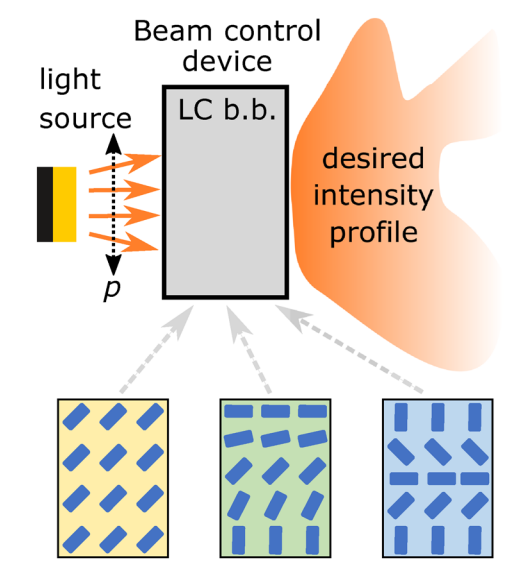
\includegraphics[width=0.30\textwidth]{images/liquidCrystalBeamSteering.png}
    \caption{Three layers of nematic liquid crystals used to deflect a light source.\autocite{zhang2023}}\label{fig:lcbeamsteering}
  \end{center}
\end{figure}

\begin{figure}[!h]
  \begin{center}
    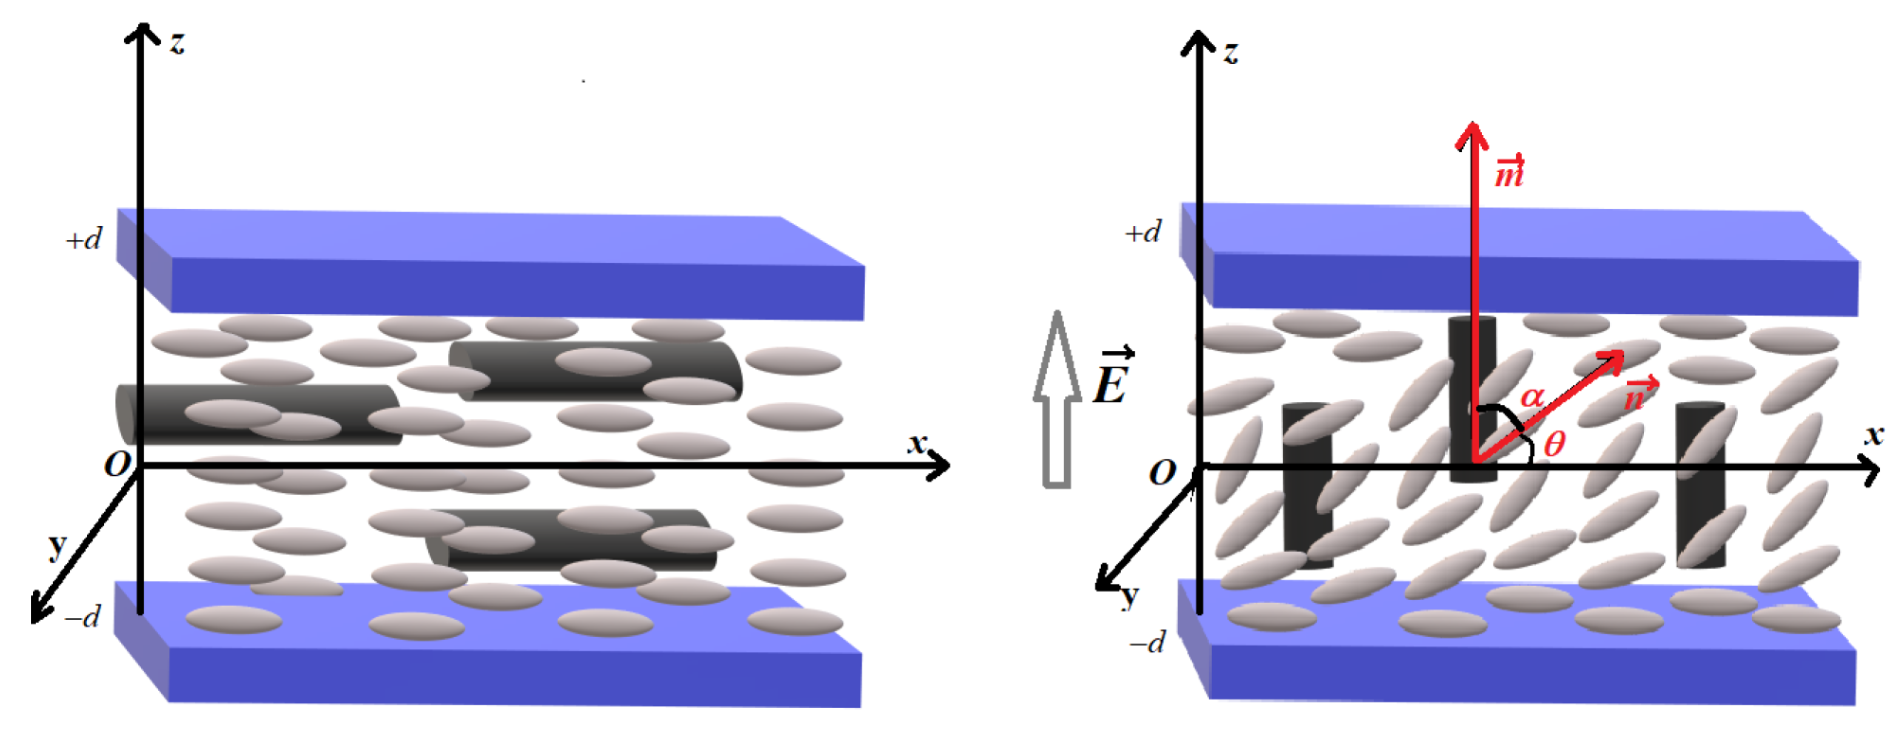
\includegraphics[width=0.70\textwidth]{images/lcelectricfield.png}
    \caption{Behavior of nematic liquid crystal cell under applied voltage. Inner molecules align strongest with the electric field, while they align more closely to the orientation of the molecules at the surface as they tend to the surface. \autocite{cirtoaje2021}}\label{fig:lcelectricfield}
  \end{center}
\end{figure}

Liquid crystals are materials with a repeated molecular structure capable of being influenced by external factors such as chemical treatment or applied electric fields.
Photons interacting with a liquid crystal interface will be refracted depending on their polarization. \autocite{cirtoaje2021}
Because the liquid crystal molecules each form an electric dipole, they orient themselves along an applied electric field as seen in Fig.~\ref{fig:lcelectricfield}
Research has shown that sub-mm layers of nematic liquid crystals can be used to achieve beam deflection at large angles when stacked upon each other. \autocite{zhang2023}
Fig.~\ref{fig:lcbeamsteering} illustrates such a configuration.
This research demonstrates that nematic liquid crystals (of a nematic molecular pattern) could be a cheaper and perhaps more viable method of realizing solid-state LiDAR.

\subsection*{PROPOSED EXPERIMENTAL DETAILS}

The chosen quadcopter platform is the \text{COEX Clover} drone, which uses open source software, ideal for our purpose. \autocite{clover}
The Clover can be integrated with any sensor thanks to its on-board Raspberry Pi 4 (RPi4); thus, we will opt to use an array of ToF sensors to measure spatial data.
This is, by definition, a LiDAR system.
The Clover supports the MAVROS protocol, which permits a communication channel between the on-board computer (RPi4) and the drone's flight controller.
The Clover also supports the \textit{Robotic Operating System} (ROS), which is a collection of software and methodologies that generalize robotics development. \autocite{ros}

\begin{figure}[!h]
  \begin{center}
    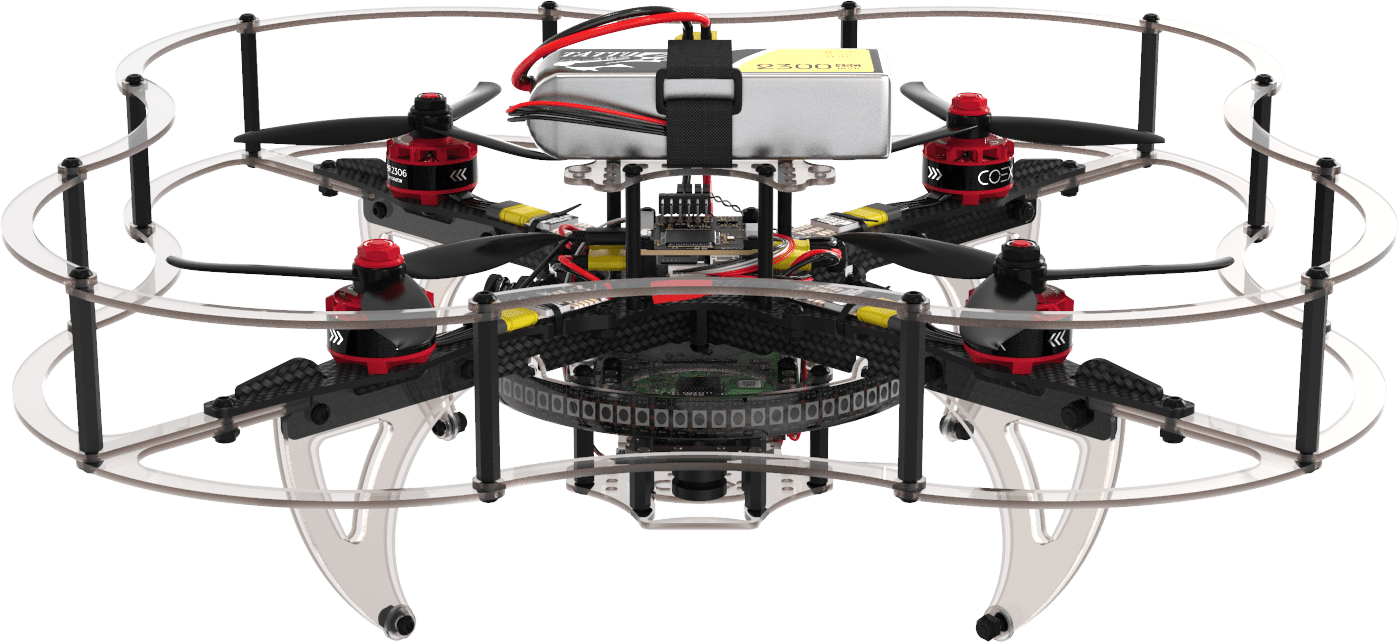
\includegraphics[width=0.40\textwidth]{images/clover.png}
    \caption{COEX Clover quadcopter. \autocite{clover}}\label{fig:clover}
  \end{center}
\end{figure}

We will start by simulating runs of the Clover using \textit{Gazebo}, a visual simulation program compatible with ROS. \autocite{gazebo}
Gazebo has a built-in physics engine, and, COEX has supplied documentation outlining how to simulate the Clover using this tool.
We will then begin to integrate DRL into this process in order to discover ways to effectively train a model for navigation.
During this stage, we will review more literature on DRL and develop a deeper understanding of the mathematics behind DRL.

As our simulations reach observable consistency, we will then consider running this model on a real-time system. This will certainly produce unexpected results, with various factors such as fluctuations in air viscosity and wind currents capable of skewing the expected behavior of a model. We will most likely spend time troubleshooting the model's control loop so that it can handle real-world conditions during this time.

Once we have a model that consistently controls the quadcopter outside of a simulation, we will focus on training the model to navigate increasingly complex environments. This will most likely be doing using iterations of arbitrary 3D shapes in a simulation. We plan to use sheets of cardboard, or some other cheap material, to create obstacles to use in our testing.

Regarding the LiDAR prototype, we plan to either use physical nematic liquid crystals (LCs) or simulate such an interaction between light and matter.
If we are to use physical nematic LCs, we will need to either purchase them or fabricate our own.
Given that the nonlinear optics lab has been left in a condition making it extremely difficult to work in, we are considering a simulation-based approach as a way to avoid the overhead of cleaning this lab in order to use it.
Nevertheless, we will explore the physics of nematic liquid crystals, specifically investigating their birefringent properties through literature, experimentation, or simulation.
After we have developed a solid understanding of how to steer an incident light source through a liquid crystal, we will begin to design a novel optical system that could be used as a component of a LiDAR system.

\subsection*{MEASURE OF SUCCESS}

During the final stages of this project, we will evaluate the effectiveness of the quadcopter in its ability to navigate through random configurations of obstacles in comparison with results found in the literature.
We will first need to determine a metric for calculating what defines the navigability of a space.
Then, we will be able to view the performance of the model with respect to the navigabililty metric to provide a quantitative evaluation of our model.

Additionally, we will look at the features of our LiDAR system to evaluate quantitative results such as maximum angle of deflection, the rate at which it could potentially measure its surroundings, and the argument that it poses as a viable technology for use in solid-state LiDAR.
Potential hurdles to a successful prototype could take the form of the following:

\begin{enumerate}
\item{Difficulty in preparing the LC samples to conform to a specific molecular configuration pattern.}
\item{A slow response time for the molecules to align to an applied magnetic field, considering that transition time is a function of the thickness of the sample. This could negatively affect the rate at which a LiDAR system could measure its surroundings if it exhibits a slow response time. \autocite{cirtoaje2021}}
\item{Finding a coherent infrared light source $(\lambda \approx 800-900\rm{nm})$}.
\end{enumerate}

\subsection*{CONCLUSION}

Autonomous systems capable of navigation will be integral to a society based upon autonomous transportation and delivery.
Exploring a current approach to training an autonomous system will allow me to shape my understanding of DRL and form a basis for working with other advanced techniques of machine learning.
Future students will be able to use the COEX Clover to do similar work as the field evolves, as this provides another platform for students to engage in robotics at Allegheny.
As solid-state LiDAR technology develops, it is important to evaluate implementations in terms of their cost, fabrication techniques, and effect on the environment.
Creating a solid-state LiDAR that uses less exotic materials and smaller components will not only make LiDAR a more accessible technology but also less harmful to the environment.

Finally, the aim of this project is to explore and evaluate the use of LiDAR sensing in the current era of robotics.
Although robotics is growing rapidly, these principles will be applicable for decades ahead, and this will work will benefit not only myself but also future students at Allegheny with an interest in autonomous systems.

\nocite{*}
\newpage

\begin{center}\small{\textbf{BIBLIOGRAPHY}}\end{center}

\printbibliography[heading=none]

\end{document}
